\documentclass[11pt, oneside]{article} 
\usepackage{geometry}
\geometry{letterpaper} 
\usepackage{graphicx}
	
\usepackage{amssymb}
\usepackage{amsmath}
\usepackage{parskip}
\usepackage{color}
\usepackage{hyperref}

\graphicspath{{/Users/telliott_admin/Dropbox/Tex/png/}}
% \begin{center} 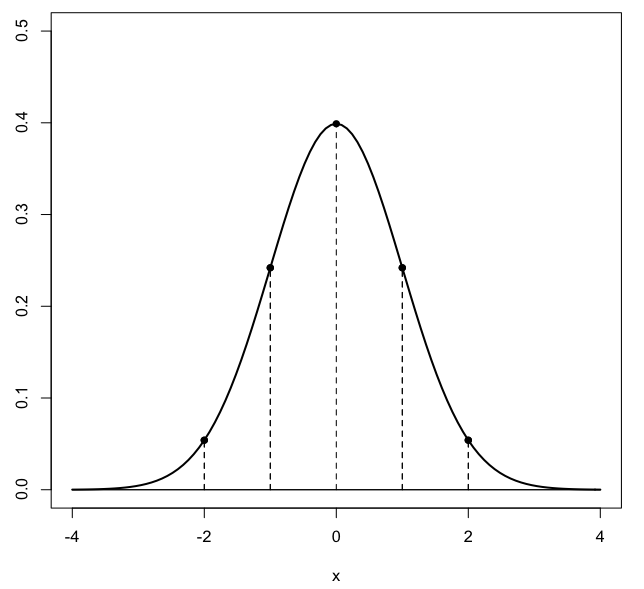
\includegraphics [scale=0.4] {gauss3.png} \end{center}

\title{Extended euclidean algorithm}
\date{}

\begin{document}
\maketitle
\Large
We break from the development of GF($2^n$) to review the Euclidean algorithm for finding the gcd of two numbers, and its "extended" version.

Let us review the method in decimal first.

Construct two co-prime integers:
\[ 3 \cdot 7 \cdot 11 = 231 \]
\[ 2 \cdot 5 \cdot 13 = 130 \]

and then carry out Euclid's algorithm, keeping the quotient as well as the remainder from each step.

\begin{verbatim}
a   b   r   q
231 130 101 1
130 101 29  1
101  29 14  3
 29  14  1  2
 14   1  0  2
\end{verbatim}
$1$ is the $GCD(130,231)$, as we already knew from listing the factors of the two numbers.

Rewrite the results as subtractions

\begin{verbatim}
  r =   a - (q)  b
101 = 231 - (1)130
 29 = 130 - (1)101
 14 = 101 - (3) 29
  1 =  29 - (2) 14
  0 =  14 - (1) 14
\end{verbatim}

One can go forward or backward.  I prefer to start from the equation with $1$ on the left-hand side:
\[ 1 = 29 - (2)14 \]

Substitute for $14$ from the previous equation:
\[ 1 = 29 - (2)[101 - (3)29] \]
\[ = (7)29 - (2)101 \]

Then substitute for $29$:
\[ 1 = (7)[130 - 101] - (2)101 \]
\[ = (7)130 - (9)101 \]

And finally, substitute for $101$:
\[ 1 = (7)130 - (9)[231 - 130] \]
\[  = (16)130 - (9)231 \]

We have thus written 1 as a \emph{linear combination} of $a$ and $b$.  

Finally, do mod $231$
\[ 1 = (16)130\ \text{mod}\ 231 \]

Our result is that $16$ and $130$ are multiplicative inverses mod $231$
\[ 9 \cdot 231 = 2079 = 16 \cdot 130 - 1 \]

There are other inverses revealed as well.

Perhaps it's obvious but still worth pointing out that every stage, we have a valid equation.  If you're in trouble, you can check that.

\subsection*{Finite field EEA}

So then the question is:  how to carry this out for a finite field like GF($2^3$)?

If we have two polynomials $a(x)$ and $b(x)$ we can find their gcd, and then find two more polynomials $s(x)$ and $t(x)$ such that
\[ gcd(a,b) = s(x)a(x) + t(x)b(x) \]

and if the gcd is 1 then they are co-prime and

\[ 1 = s(x)a(x) + t(x)b(x) \]

So if $a(x) = m(x)$ is the irreducible polynomial $1011$, then certainly the gcd with any polynomial in the field is 1 so we should be able to find

\[ 1 = s(x)m(x) + t(x)b(x) \]

and then do modulo $m = 1011$ we have

\[ 1 = t(x)b(x) \]

I have been unable to find a source on the web for this, so I am just trying things.  In decimal, the choice of the factor (that we call the quotient $q$ of $a$ below, where $qb = a$) is unambiguous.  This is not so in our system.  Instead, all we require is that the degree of the resulting $qb$ be the same as $a$.  Sometimes one choice leads to a result more rapidly than another.

So far as I am aware, all choices for q that give the right degree lead to the correct result.

\subsection*{example 1: $ x^2 + x$}
Recall that $x^2 + x$ is written as 110   I'm going to adopt the convention that elements of the field (degree 2 or less) will be written with as few digits as possible.

We seek gcd($1011$,$110$).  The smallest $q$ that works is $10$:
\begin{verbatim}
   a   b   q   qb   r
1011 110  10 1100 111
 110 111  01  111   1
------
111 = 1011 - 10 * 110
  1 =  110 - 01 * 111
    =  110 - 01[1011 - 10 * 110]
    =  11 * 110
    = (x + 1)(x^2 + x)
\end{verbatim}

Note $q \cdot b > a$ is still OK.

Suppose we try $q = 11$:
\begin{verbatim}
   a   b   q   qb   r
1011 110  11 1010   1
------
  1 =  1011 - 11 * 110
    =  11 * 110
    = (x + 1)(x^2 + x)
\end{verbatim}

We have that the multiplicative inverse of $x^2 + x$ is $x + 1$, which should not come as a surprise.

\[ (x^2 + x)(x + 1) = x^3 + x^2 + x^2 + x \]
\[ = x^3 + 1 \]
\[ = (x + 1) + x = 1 \]

\subsection*{example 2: $x$}
We want gcd($1101, 010$).  

We might pick $q = 100$ but notice $q = 101$ gives
\begin{verbatim}
   a   b   q   qb   r
1011 010 101 1010   1
------
  1 = 1011 - 101 * 010
    =  101 * 010
    =  (x^2 + 1)(x)
\end{verbatim}

Refer back to above to the multiplication table or the logarithms section to confirm that $x$ and $x^2 + 1$ are inverses.  Does $q = 100$ work?

\begin{verbatim}
   a   b   q   qb   r
1011 010 100 1000  11
  10  11   1   11   1
------
 11 = 1011 - 100 * 010
  1 =   10 - 1 * 11
    =   10 - 1 * [1011 - 100 * 010]
    =  101 * 010
    =  (x^2 + 1)(x)
\end{verbatim}

The answer is the same, $x^2 + 1$ and $x$ are inverses.

\subsection*{example 3: $x^2 + x + 1$}

\begin{verbatim}
gcd(m, x^2 + x + 1)

   a   b   q   qb   r
1011 111  10 1110 101
 111 101   1  101  10
 101  10  10  100   1

101 = 1011 - (10)111
 10 =  111 - (01)101
  1 =  101 - (10)10
    =  101 - (10)[111 - (01)101]
    =  (11)101 - (10)111
    =  (11)[1011 - (10)111] - (10)111
    = -(110)111 - (10)111
    =  (100)111
    = (x^2)(x^2 + x + 1)
\end{verbatim}

Suppose we made a different choice for that first quotient:

\begin{verbatim}
gcd(m, x^2 + x + 1)

   a   b   q   qb   r
1011 111  11 1001  10
 111  10  11  110   1

  10 = 1011 - (11)111
   1 = 111  - (11)10
     = 111 - (11)[1011 - (11)111]
     = 111 + (101)111 
     = 100(111)
     = (x^2)(x^2 + x + 1)
\end{verbatim}

Provisionally, it seems that one can pick any multiplier that will get the degree right, and we obtain the correct answer.

\end{document}
